% Lecture Template for ME3050 - Dynamic Modeling and Controls - Tennessee Technological University
% Spring 2023 - condensing and streamlining lectures by combining topics into a single PDF under the module name
% this will simplify file and link management as well as make lectures easier to use in class
% - added image/ to clean directory and reduce redundancy, specific to module for now  

% Module Name: - Introduction
% Topic 1 - Components, Units, and Symbols
% Topic 2 - Fundamental Laws
% Topic 3 - Circuit Applications

\documentclass[fleqn]{beamer} % for presentation (has nav buttons at bottom)

%\usepackage{/home/tntech.edu/thill/courses/measurements/lectures/measurements_lectures}
\usepackage{/home/thill/courses/measurements/lectures/measurements_lectures}
%\usepackage{/mnt/c/Users/thill/Documents/courses/measurements/lectures/measurements_lectures}

\author{ME3050 - Dynamics Modeling and Controls}

\newcommand{\MNUM}{1\hspace{2mm}} % module number 
\newcommand{\moduletitle}{Introduction}

\newcommand{\sectionItitle}{System Dynamics}
\newcommand{\sectionIItitle}{Units and Conversions}
\newcommand{\sectionIIItitle}{Models and Assumptions}

\newcommand{\sectionIsubsectionItitle}{Definition of Dynamics}
\newcommand{\sectionIsubsectionIItitle}{Modeling and Analysis}
\newcommand{\sectionIsubsectionIIItitle}{Model Based Design}
\newcommand{\sectionIsubsectionIVtitle}{Course Topics}

\newcommand{\sectionIIsubsectionItitle}{Standard Units}
\newcommand{\sectionIIsubsectionIItitle}{Unit Conversions}
\newcommand{\sectionIIsubsectionIIItitle}{Frequency and Circular Frequency}
\newcommand{\sectionIIsubsectionIVtitle}{Example - Units Matter}

\newcommand{\sectionIIIsubsectionItitle}{Mathematical Modeling}
\newcommand{\sectionIIIsubsectionIItitle}{Solid Mechanics and Dynamics}
\newcommand{\sectionIIIsubsectionIIItitle}{Thermal and Fluid Systems}
\newcommand{\sectionIIIsubsectionIVtitle}{Electrical and Power Systems}

\newcommand{\btVFill}{\vskip0pt plus 1filll}

% custom box
\newsavebox{\mybox}

\title{Lecture Module - \moduletitle}

\date{Mechanical Engineering\vspc Tennessee Technological University}

\begin{document}

	\lstset{language=MATLAB,basicstyle=\ttfamily\small,showstringspaces=false}

	\frame{\titlepage \center\begin{framed}\Large \textbf{Module \MNUM - \moduletitle}\end{framed} \vspace{5mm}}

	% Module Outline
	\begin{frame} 
		\large \textbf{Module \MNUM - \moduletitle} \vspace{3mm}\\

		\begin{itemize}
			\item Topic 1 - \hyperlink{sectionI}{\sectionItitle} \vspc % section I
			\item Topic 2 - \hyperlink{sectionII}{\sectionIItitle} \vspc % section II
			\item Topic 3 - \hyperlink{sectionIII}{\sectionIIItitle} \vspc % section III
		\end{itemize}

	\end{frame}

	% section I
	\section{\sectionItitle}\label{sectionI}

		% section I Outline
		\begin{frame} 
			\large \textbf{Topic 1 - \sectionItitle} \vspace{3mm}\\

			\begin{itemize}
				\item \hyperlink{sectionIsubsectionI}{\sectionIsubsectionItitle} \vspc %  section I subsection I
				\item \hyperlink{sectionIsubsectionII}{\sectionIsubsectionIItitle} \vspc % section I subsection II
				\item \hyperlink{sectionIsubsectionIII}{\sectionIsubsectionIIItitle} \vspc % section I subsection III
				\item \hyperlink{sectionIsubsectionIV}{\sectionIsubsectionIVtitle} \vspc % section I subsection IV
			\end{itemize}
		\end{frame}
		
		% section I subsection I 
		\subsection{\sectionIsubsectionItitle}\label{sectionIsubsectionI}

			\begin{frame}
				\frametitle{\sectionIsubsectionItitle}
				\bigskip

				\large
				Dynamics is ...\vspcc

				the study of how moving objects behave, \vspcc
				or \vspcc
				an area of mechanics that studies movement and its causes,\vspcc
				or \vspcc
				%\Large{"The dynamical system concept is a mathematical formalization for any fixed "rule" which describes the time dependence of a point's position in its ambient space. "} \vspace{5mm} \\

				{\it system dynamics} is the study of {\bf modeling} and {\bf analysis} of dynamical systems as a function of time.\vspc

				\btVFill
			\end{frame}

			\begin{frame}
				\frametitle{\sectionIsubsectionItitle}
				\bigskip

				\frametitle{Dynamics vs System Dynamics}

				\large
				Dynamics: find state of \underline{object} at \underline{a specific instant in time} \vspccc

				System Dynamics: find state of \underline{system} as a \underline{function of time}  \vspc

				$\rightarrow$ Leads to use of differential equations. $m\ddot{x}+c\dot{x}+kx=f(t)$

				\btVFill
			\end{frame}

		% section I subsection II
		\subsection{\sectionIsubsectionIItitle}\label{sectionIsubsectionII}

			\begin{frame}
				\frametitle{\sectionIsubsectionIItitle}
				\bigskip
				%\frametitle{What is Mathematical Modeling?}

				A mathematical model is a description of a system using mathematical concepts and language. The process of developing a mathematical model is termed mathematical {\bf modeling} ... \vspc
				...  used in the natural sciences and engineering disciplines ...  \href{https://en.wikipedia.org/wiki/Mathematical_model}{\tiny Wikipedia}

				\begin{itemize}
					\item Model Simplification
					\item Force and Loading Analysis with FBDs
					\item Fundamental Laws Lead to Equations of Motion
					\item Newton's Second Law and Conservation of Energy
				\end{itemize}

				\btVFill
			\end{frame}

				%\btVFill
			\begin{frame}
				\frametitle{\sectionIsubsectionIItitle}
				\bigskip
				%\frametitle{What is Analysis?}

				{\bf Analysis} is the process of breaking a complex topic or substance into smaller parts in order to gain a better understanding of it... \href{https://en.wikipedia.org/wiki/Analysis}{\tiny Wikipedia}

				\begin{itemize}
					\item Study Model to find System Response
					\item Time-Domain analysis: examine system response in time to various inputs and initial conditions
					\item Frequency-Domain analysis: examine system response when subject to sinusoidal inputs
				\end{itemize}
		
				\btVFill
			\end{frame}

			\begin{frame}
				\frametitle{sectionIsubsectionIIItitle}
				\bigskip

				Model-Based Design (MBD) is a mathematical and visual method of addressing problems associated with designing complex control, signal processing and communication systems. It is used in many motion control, industrial equipment, aerospace, and automotive applications... \href{https://en.wikipedia.org/wiki/Model-based_design}{\tiny Wikipedia}

				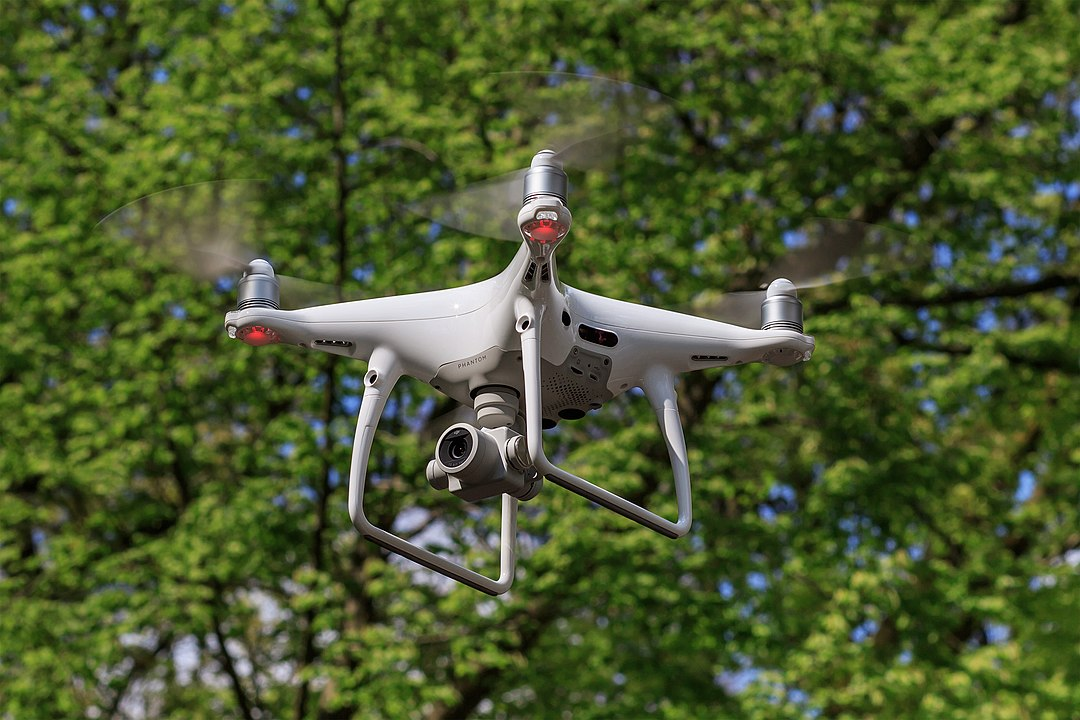
\includegraphics[scale=.08]{images/dji_phantom_fig2.jpg}\hspccc
				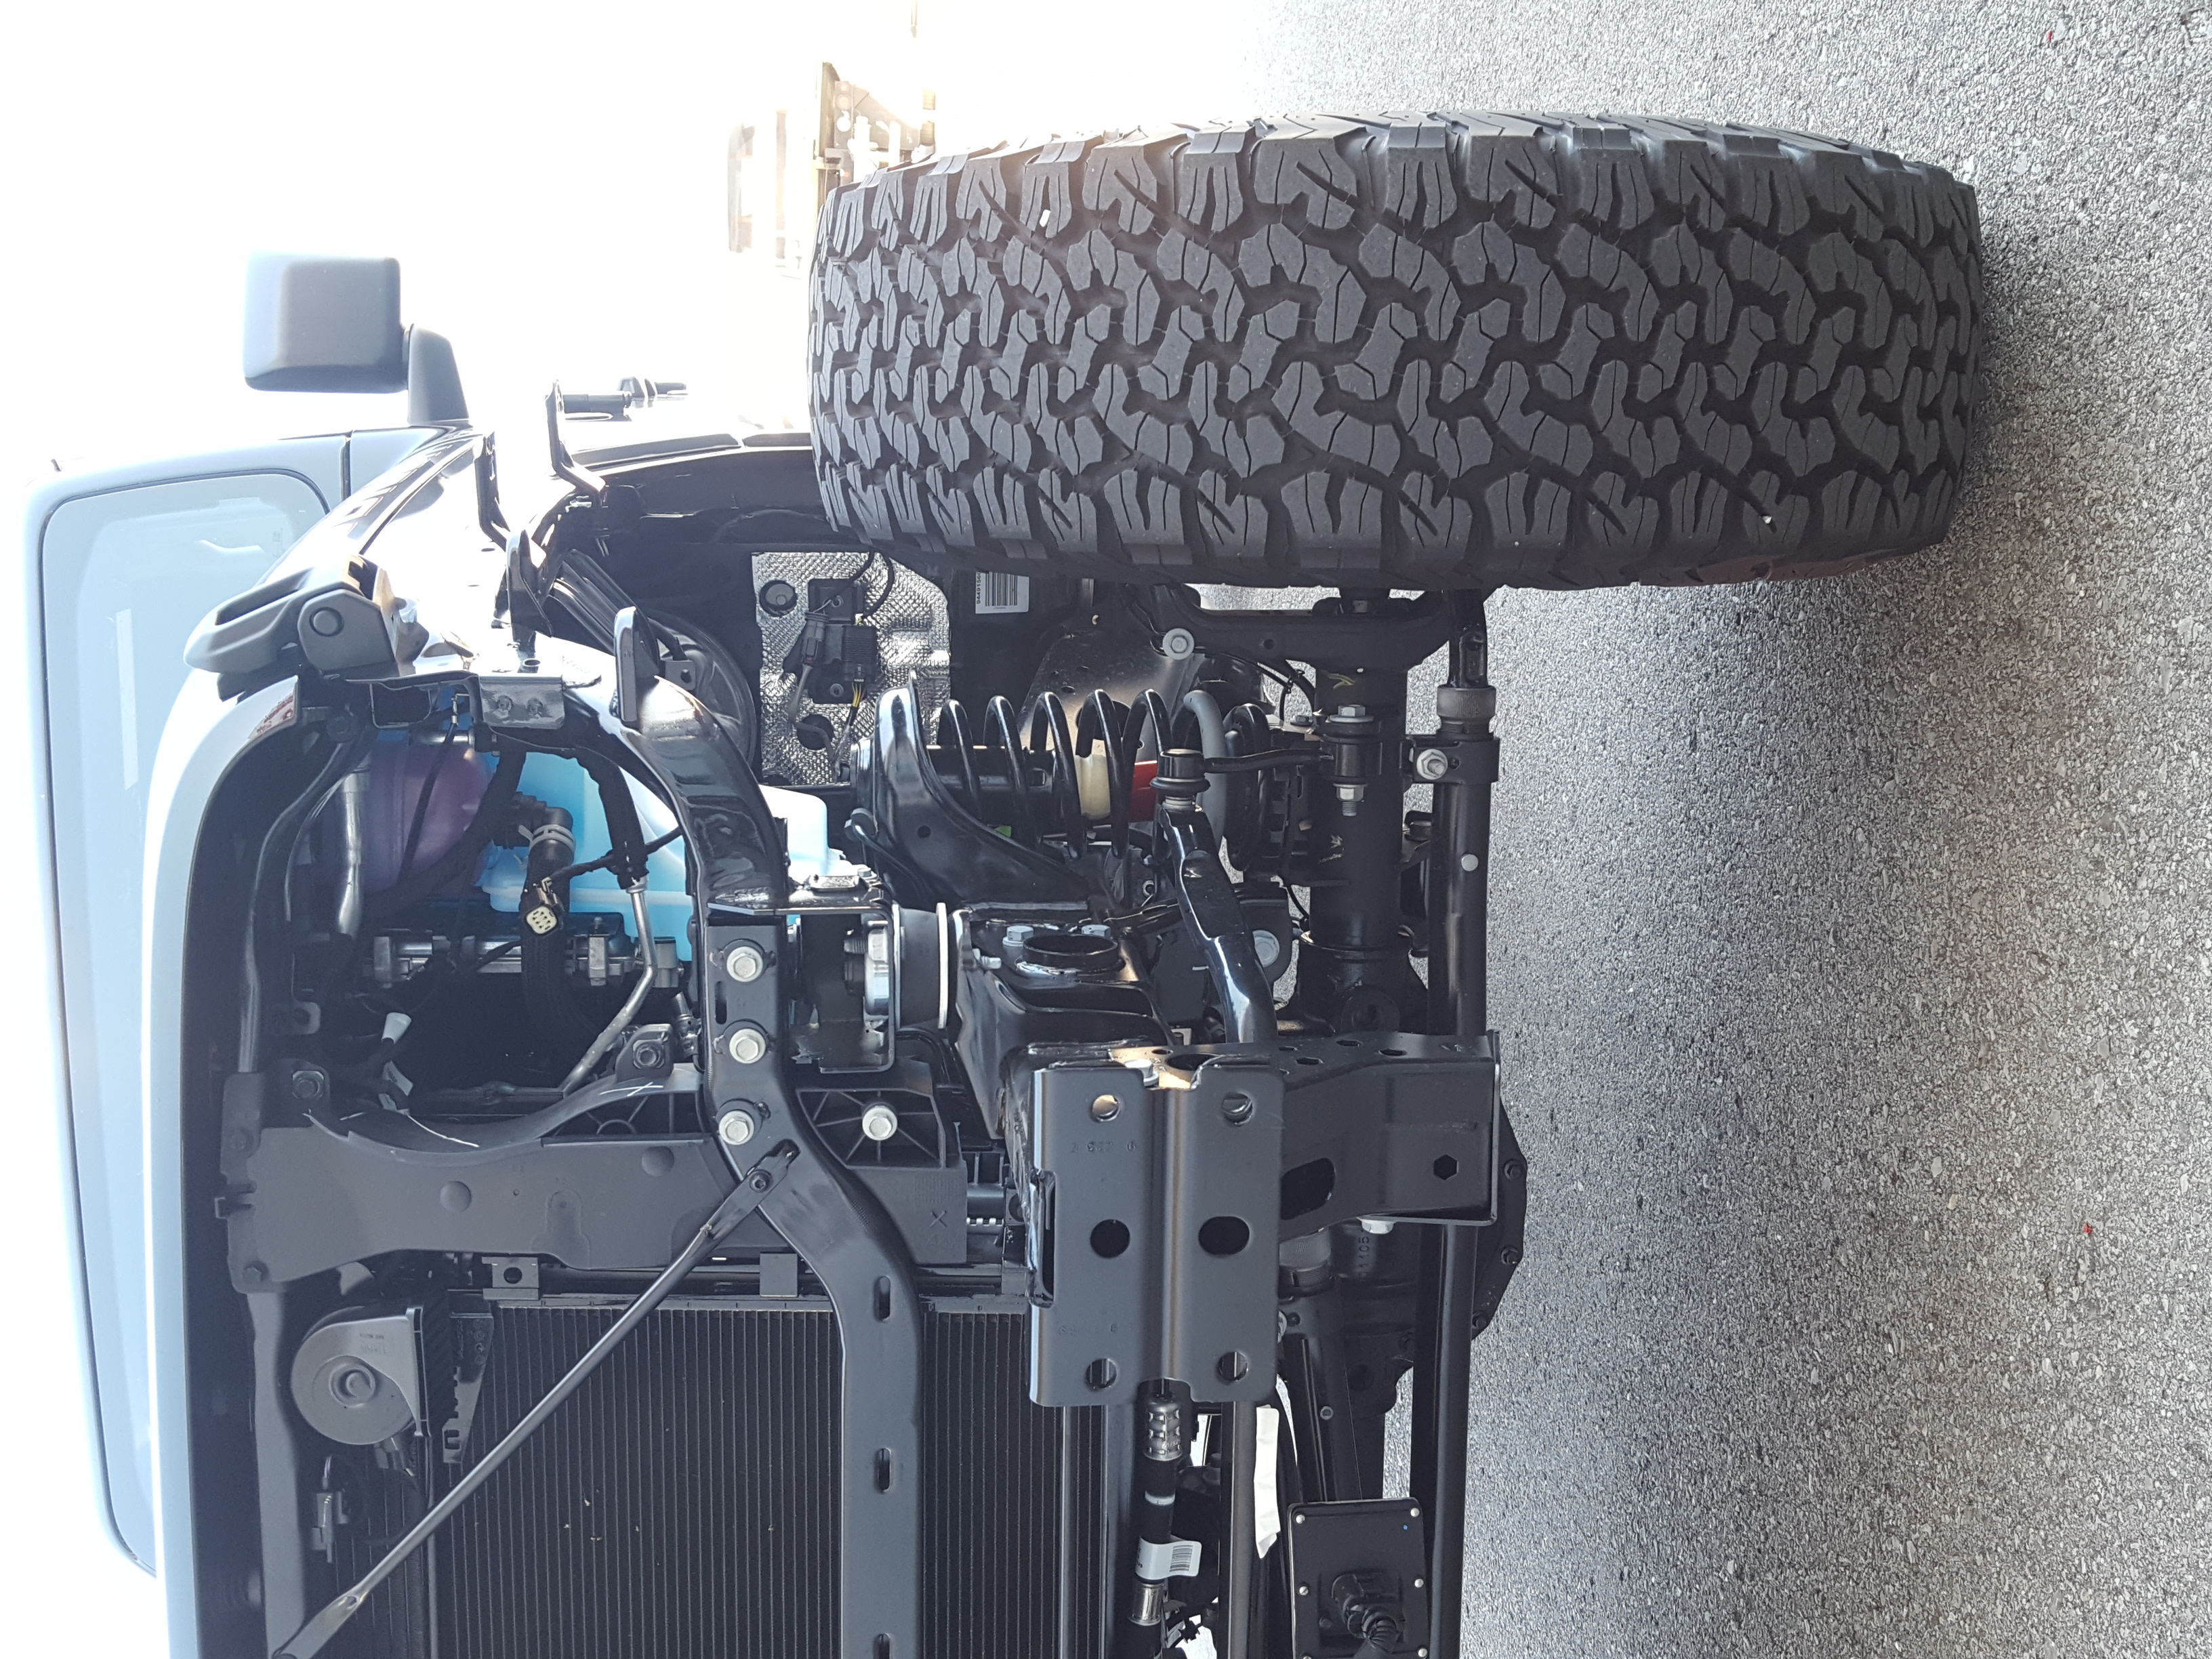
\includegraphics[scale=.025,angle=-90,origin=c]{images/jeep_01.jpg} \hspccc
				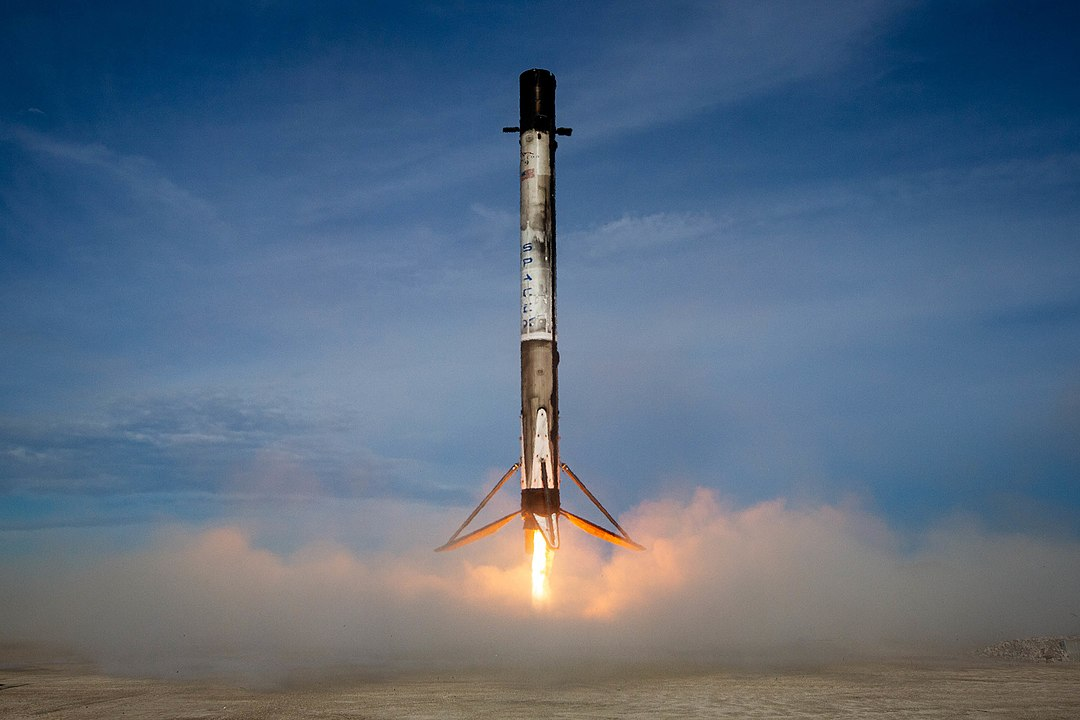
\includegraphics[scale=.1]{images/falcon9_fig2.jpg} \\
				{\tiny\href{https://en.wikipedia.org/wiki/Phantom_(UAV)}{Image: Wikipedia} \hspace{20mm}Image: TH \hspace{20mm}\href{https://en.wikipedia.org/wiki/SpaceX\#/media/File:CRS-18_Mission_(48380511427).jpg}{Image: Wikipedia} }

				\btVFill
			\end{frame}


		% section I subsection III
		\subsection{\sectionIsubsectionIIItitle}\label{sectionIsubsectionIII}
			\begin{frame} 
				\frametitle{\sectionIsubsectionIIItitle}
				%\bigskip
		

				%\btVFill
			\end{frame}	

			\begin{frame} 
				\frametitle{\sectionIsubsectionIIItitle}
				%\bigskip
		

				%\btVFill
			\end{frame}	

		% section I subsection IV
		\subsection{\sectionIsubsectionIVtitle}\label{sectionIsubsectionIV}	

			\begin{frame}
				\frametitle{\sectionIsubsectionIVtitle}
				%\bigskip
		

				%\btVFill
			\end{frame}

			\begin{frame}
				\frametitle{\sectionIsubsectionIVtitle}
				%\bigskip
		

				%\btVFill
			\end{frame}

	
	% Section II
	\section{\sectionIItitle}\label{sectionII}

		% section II Outline
		\begin{frame}
			\large \textbf{Topic 2 - \sectionIItitle} \vspace{3mm}\\

			\begin{itemize}
				\item \hyperlink{sectionIIsubsectionI}{\sectionIIsubsectionItitle} \vspc %  section II subsection I
				\item \hyperlink{sectionIIsubsectionII}{\sectionIIsubsectionIItitle} \vspc % section II subsection II
				\item \hyperlink{sectionIIsubsectionIII}{\sectionIIsubsectionIIItitle} \vspc % section II subsection III
				\item \hyperlink{sectionIIsubsectionIV}{\sectionIIsubsectionIVtitle} \vspc % section II subsection IV
			\end{itemize}

		\end{frame}

		% section II subsection I
		\subsection{\sectionIIsubsectionItitle}\label{sectionIIsubsectionI}

			\begin{frame}[label=sectionIIsubsectionI]
				\frametitle{\sectionIIsubsectionItitle}
				%\bigskip
		

				%\btVFill
			\end{frame}

		    \begin{frame}[label=sectionIIsubsectionI]
				\frametitle{\sectionIIsubsectionItitle}
				%\bigskip
		

				%\btVFill
			\end{frame}	

		% section II subsection II
		\subsection{\sectionIIsubsectionIItitle}\label{sectionIIsubsectionII}

			\begin{frame}
				\frametitle{\sectionIIsubsectionIItitle}
				%\bigskip
		

				%\btVFill
			\end{frame}

		% section II subsection III
		\subsection{\sectionIIsubsectionIIItitle}\label{sectionIIsubsectionIII}

			\begin{frame}
				\frametitle{\sectionIIsubsectionIIItitle}
				%\bigskip
		

				%\btVFill
			\end{frame}

			\begin{frame}
				\frametitle{\sectionIIsubsectionIIItitle}
				%\bigskip
		

				%\btVFill
			\end{frame}

			\begin{frame}
				\frametitle{\sectionIIsubsectionIIItitle}
				%\bigskip
		

				%\btVFill
			\end{frame}

		% section II subsection IV 
		\subsection{\sectionIIsubsectionIVtitle}\label{sectionIIsubsectionIV}

			\begin{frame}
				\frametitle{\sectionIIsubsectionIVtitle}
				%\bigskip
		

				%\btVFill
			\end{frame}

			\begin{frame}
				\frametitle{\sectionIIsubsectionIVtitle}
				%\bigskip
		

				%\btVFill
			\end{frame}
		
	% Section III
	\section{\sectionIIItitle}\label{sectionIII}

		% section III Outline
		\begin{frame}
			\large \textbf{Topic 3 - \sectionIIItitle} \vspace{3mm}\\

			\begin{itemize}
				\item \hyperlink{sectionIIIsubsectionI}{\sectionIIIsubsectionItitle} \vspc %  section III subsection I
				\item \hyperlink{sectionIIIsubsectionII}{\sectionIIIsubsectionIItitle} \vspc % section III subsection II
				\item \hyperlink{sectionIIIsubsectionIII}{\sectionIIIsubsectionIIItitle} \vspc % section III subsection III
				\item \hyperlink{sectionIIIsubsectionIV}{\sectionIIIsubsectionIVtitle} \vspc % section III subsection IV
			\end{itemize}

		\end{frame}

		% section III subsection I
		\subsection{\sectionIIIsubsectionItitle}\label{sectionIIIsubsectionI}

			\begin{frame}
				\frametitle{\sectionIIIsubsectionItitle}
				%\bigskip
		

				%\btVFill
			\end{frame}

			\begin{frame}
				\frametitle{\sectionIIIsubsectionItitle}
				%\bigskip
		

				%\btVFill
			\end{frame}

		% section III subsection II
		\subsection{\sectionIIIsubsectionIItitle}\label{sectionIIIsubsectionII}	

			\begin{frame}
				\frametitle{\sectionIIIsubsectionIItitle}
				%\bigskip
		

				%\btVFill
			\end{frame}

		% section III subsection III
		\subsection{\sectionIIIsubsectionIIItitle}\label{sectionIIIsubsectionIII}

			\begin{frame}
				\frametitle{\sectionIIIsubsectionIIItitle}
				%\bigskip
		

				%\btVFill
			\end{frame}

			\begin{frame}
				\frametitle{\sectionIIIsubsectionIIItitle}
				%\bigskip
		

				%\btVFill
			\end{frame}

		% section III subsection IV
		\subsection{\sectionIIIsubsectionIVtitle}\label{sectionIIIsubsectionIV}	

			\begin{frame}
				\frametitle{\sectionIIIsubsectionIVtitle}
				%\bigskip
		

				%\btVFill
			\end{frame}

			\begin{frame}
				\frametitle{\sectionIIIsubsectionIVtitle}
				%\bigskip
		

				%\btVFill
			\end{frame}

\end{document}





